\chapter{Metodologia}
\label{chp:metodologia}

\section{Métodos Mistos}
A abordagem escolhida durante a elaboração deste trabalho foi a de Métodos Mistos de pesquisa, a qual consiste em combinar análise qualitativa com análise quantitativa.

A principal diferença entre esses dois métodos de pesquisa é que a quantitativa é padronizada, baseada em escalas numéricas e analíticas, cuja estratégia utilizada neste trabalho foi a coleta de dados por meio de questionário online. Enquanto a pesquisa qualitativa tem base no caráter subjetivo, usando narrativas escritas ou faladas, neste trabalho foram utilizadas entrevistas como forma de coleta e mensuração.\citep{saldana2011fundamentals}

\section{Estudo 1 - Pesquisa Qualitativa}

\subsection{Motivação}

Este estudo selecionou participantes de Hackathons, os quais não terão suas identidades reveladas por questões éticas, como objeto de análise. Também, por conveniência atendendo o seguinte critério:
\begin{itemize}
    \item Participaram de eventos de hackathons nos últimos anos;
\end{itemize}

A motivação para os critérios pré estabelecidos foi encontrar pessoas engajadas e com experiência em participação para lucidar o tema desta pesquisa.

Com abordagens diferentes de coleta e análise de dados, este estudo qualitativo buscou captar a percepção das pessoas no tocante à abordagem de propriedade intelectual nos eventos de hackathon que participaram. Mas especificamente em relação à ceder ou não, dependendo do tipo de hackathon; entender a importância, na concepção dos entrevistados, dos direitos à propriedade intelectual nos eventos; e a confiança que eles têm ao participar de hackathons e o destino de seus códigos.

\subsection{Amostra}

Inicialmente, foram escolhidas pessoas que participaram de eventos de hachathon, atendendo assim o critério especificado na seção Motivação deste estudo, assim seria mais provável encontrar pessoas dispostas a falarem sobre a cessão ou não dos direitos à PI. Foram selecionadas quatro entrevistas para o estudo, sendo elas duas pessoas que venceram hackathons e duas que apenas participaram delas. A partir daqui iremos referenciar essas pessoas como \textbf{"Cederam PI"} e \textbf{"Não Cederam"} para proteger as identidades das mesmas, conforme pode ser visto na \autoref{tab:categorizarParticipantes}. 

%TABELA CATEGORIZANDO OS PARTICIPANTES
\begin{table}[H]
\centering
\caption{Dados dos Entrevistados}
\label{tab:categorizarParticipantes}
\begin{tabular}{lp{2.8cm}p{2.8cm}|p{2.8cm}p{2.8cm}}
                                  & \multicolumn{2}{c|}{\textbf{Cederam PI}} & \multicolumn{2}{c}{\textbf{Não Cederam}} \\
 &
  \multicolumn{1}{c}{\textbf{Entrevistado 1}} &
  \multicolumn{1}{c|}{\textbf{Entrevistado 2}} &
  \multicolumn{1}{c}{\textbf{Entrevistado 3}} &
  \multicolumn{1}{c}{\textbf{Entrevistado 4}} \\ \hline
\multicolumn{1}{l|}{Formação}     & Médio Completo      & Médio Completo     & Médio Completo      & Médio Completo     \\
\multicolumn{1}{l|}{Curso Atual} &
  Eng. da Computação &
  Eng. da Computação &
  Eng. da Computação &
  Eng. da Computação \\
\multicolumn{1}{l|}{Cargo}        & Desenvolvedor       & Desenvolvedor      & Analista            & Bolsista           \\
\multicolumn{1}{l|}{Idade}        & 23                  & 23                 & 22                  & 20                 \\
\multicolumn{1}{l|}{Gênero}       & Masculino           & Masculino          & Feminino            & Masculino          \\
\multicolumn{1}{l|}{Naturalidade} & Recife              & Recife             & Recife              & Recife     \\
\multicolumn{1}{l|}{Qtd. Hackathons} & 2                   & 3-4                & 1                   & 2                        
\end{tabular}
\end{table}

Todos os participantes foram esclarecidos das motivações da pesquisa e do caráter confidencial de sua contribuição. Foi assinado um Termo de Consentimento (disponível para consulta no \autoref{ap:termoConcent}).

% Eventos os quais participaram, descrever alguns
% Percepções pessoais dos eventos

\subsection{Coleta de Dados}

Para este estudo, a coleta de dados se deu principalmente por meio de entrevistas semiestruturadas (cujo roteiro pode ser consultado no \autoref{ap:entrevista}) com os participantes. As entrevistas foram gravadas na íntegra (áudio) e algumas notas foram tomadas em tempo real. Dentre as 4 entrevistas realizadas, todas foram presenciais.


\subsection{Análise de Dados}


Após o levantamento de todos os dados através das entrevistas semiestruturadas, foi analisado os materiais pelas categorizações referenciadas anteriormente. Primeiramente foi analisados o material referente aos que cederam sua PI nos eventos. Após a primeira análise, a metodologia foi repetida para os participantes que não cederam sua PI. Dessa forma os contextos ficaram mais isolados. Por fim pôde-se montar os perfis a partir da visão dos participantes.

Os áudios foram ouvidos integralmente, para que pudesse ser criado cada perfil a fim de compor uma ideia inicial. Os mesmos foram transcritos, para coletar notas de falas relevantes e capturando os códigos. \citep{saldana2011fundamentals}

Saldaña define um código como sendo simbolicamente atribuído a um atribulo sumativo ou evocativo para uma porção de dados qualitativos. \citep{saldana2011fundamentals}

Assim foram atribuídos códigos para cada tema encontrado nos transcritos como descritos por \citet{lakatos2017tecnicas}. \citet{saldana2015coding} também descreve como são gerados alguns códigos e que não existe ciência exata para gerá-los, e sim intuitividade e prática ao ler e reler as transcrições para identificar cada código ou tema utilizado na pesquisa. Foi utilizado um método de comparação constante através da codificação \textit{in vivo}, também conhecida como codificação literal ou codificação natural. \citet{saldana2015coding}

Também foi realizado uma nuvem de palavras geral com todas as palavras dos entrevistados e nuvens individuais, as quais ajudaram a para obter \textit{insights} imediatos sobre os termos mais importantes para os códigos, conforme podem ser vistos no \autoref{ap:nuvem}

Após as primeiras leituras nas transcrições dos que cederam PI e nos que não cederam PI, capturando e validando os códigos, encontrou-se cinco temas/categorias principais, os quais serão melhor descritos na seção de resultados. 





%%%%%%%%%%%%%%%%%%%%%%%%%%%%%%%%%%%%%%%%%%%%%%%%%%%%%%%%%%%%%


\section{Estudo 2 - Pesquisa Quantitativa}

A pesquisa quantitativa nos ajuda a entender as informações coletadas e dimensioná-las e com o intuito de quantificar opiniões e informações para o estudo proposto.
Sua maior motivação é avaliar com maior foco (mas não exclusivamente) questões sobre a relevância de alguns pontos descritos em regulamentos de eventos de hackathons, clareza de conteúdo dos mesmos, também sobre cessão de direitos e respeito dos mesmos em um determinado evento, passando ainda pelas dimensões de escolaridade, idade e naturalidade. 

Ao capturar essas informações, queremos compreender e enfatizar o raciocínio lógico e todas as informações que se possam mensurar sobre a percepção dos participantes em eventos de hackathon no tocante à propriedade intelectual.

\subsection{Estrutura}

Um questionário utilizando a ferramenta do Google Forms\footnote{ Google Forms <https://www.google.com/forms/about/> 
} foi elaborado para coleta das informações, com 20 perguntas, o questionário encontra-se no \autoref{ap:questionario}. As questões foram elaboradas da seguinte forma:
\begin{itemize}
   \item 1 pergunta para saber se o participante já realizou ou não uma hackathon
   \item 4 perguntas de caráter pessoal, para entender o perfil do participante
   \item 4 perguntas para o entendimento entre o participante e o regulamento da(s) hackathons
   \item 10 perguntas para capturar o entendimento entre o participante e a propriedade intelectual em eventos de hackathons
   \item 1 pergunta para entender a opinião do participante com relação ao assunto
     
\end{itemize}
   
O questionário possui, em sua maioria, perguntas fechadas, onde as abertas foram colocadas como facultativas, com exceção da idade, cidade onde reside e quantidade de participações em hackathons. A tabela abaixo expressa quais os métodos aplicados em cada pergunta, assim como o objetivo ao aplicar cada um dos métodos citados.
%%%%%%%%%%%%%%%%%%%%%%%%%%%%%%%%%%%%%%%%%%%%%%%%%%%%%%%
\begin{table}[H]
\centering
\caption{Questionário Online}
\label{tab:questionario}
\begin{tabular}{|l|l|p{6,7cm}|}
\hline
\textbf{PERGUNTAS}      & \textbf{MÉTODO APLICADO} & \textbf{OBJETIVO}                                                                                                     \\ \hline
1ª                      & Dicotômica               & Filtrar apenas as pessoas que participaram de Hackathons                                                              \\ \hline
2ª - 5ª                 & Resposta Única           & Entender perfil pessoal e geográfico do participante                                                                  \\ \hline
6ª                      & Resposta Única           & Mensurar a quantidade de Hackathons participadas                                                                      \\ \hline
7ª                      & Múltipla Escolha         & Mensurar quantos leem o regulamento                                                                                   \\ \hline
8ª                      & Resposta Aberta          & Entender a motivação para o participante estar no evento                                                              \\ \hline
9ª                      & Ranking                  & Ranquear os tópicos do mais ao menos importante pela ótica do participante                                            \\ \hline
10ª, 11ª, 17ª, 18ª      & Escala de Likert 1-5     & Entender de forma mais palpável a mensuração dos participantes com relação à concordância ou não dos pontos abordados \\ \hline
12ª, 13ª, 15ª, 16ª, 19ª & Dicotômica               & Compreender a mentalidade do participante com relação ao questionário                                                 \\ \hline
14ª                     & Múltipla Escolha         & Medir o grau de percepção do participante sob uma lista de aspectos                                                   \\ \hline
20ª                     & Resposta Aberta          & Expressar a opinião mais aberta do participante quanto ao assunto                                                     \\ \hline
\end{tabular}
\end{table}


\subsection{Procedimento}

Após o termino do formulário online na plataforma Google Forms, juntamente com uma breve introdução relacionada à motivação da pesquisa, a privacidade e ao voluntariado da resposta. 

Em seguida, o questionário foi largamente divulgado nas redes sociais tais como: Whatsapp\footnote{ WhatsApp <https://www.whatsapp.com/> } e Telegram\footnote{ Telegram <https://telegram.org/>}, grupos e páginas da rede social Facebook\footnote{ Facebook <https://www.facebook.com>} seja eles universitários ou de eventos de hackathons, grupos de emails institucionais e universitários, baseados em linguagens programacionais e eventos de hackathon, além da rede social Reddit\footnote{ Reddit <https://www.reddit.com/>}. 


\subsection{Amostra}

Num período de 4 (quatro) meses online, durante o mês de novembro de 2019 até março de 2020, o questionário obteve 174 respostas, das quais 78 (44,82\%) responderam que participaram de hackathons. 
O perfil dos participantes está detalhado na tabela X. Com média de idade de 26,8 anos e (desvio padrão = 9,20), a idade dos participantes variou entre 18 e 85 anos e faixa etária modal de 18 a 23 anos. Compreendendo, em sua maioria, pessoas que se identificam com o gênero masculino, cerca de 79,49\%.

\begin{table}[H]
\centering
\caption{Dados demográficos do Estudo Quantitativo}
\label{tab:dados-demo}
\begin{tabular}{lcc}
\rowcolor[HTML]{FFFFFF} 
                                                                   & \textbf{RESPOSTAS} & \textbf{\% do TOTAL} \\ \hline
\rowcolor[HTML]{EFEFEF} 
\multicolumn{1}{l|}{\cellcolor[HTML]{FFFFFF}\textbf{IDADE (ANOS)}} &                    &                      \\
\rowcolor[HTML]{FFFFFF} 
\multicolumn{1}{l|}{\cellcolor[HTML]{FFFFFF}Entre 18 e 23}         & 33                 & 42,31                \\
\rowcolor[HTML]{EFEFEF} 
\multicolumn{1}{l|}{\cellcolor[HTML]{FFFFFF}Entre 24 e 30}         & 28                 & 35,90                \\
\rowcolor[HTML]{FFFFFF} 
\multicolumn{1}{l|}{\cellcolor[HTML]{FFFFFF}Entre 31 e 36}                 & 8                  & 10,25                \\
\rowcolor[HTML]{EFEFEF} 
\multicolumn{1}{l|}{\cellcolor[HTML]{FFFFFF}Entre 37 e 41}                 & 6                  & 7,69                 \\
\rowcolor[HTML]{FFFFFF} 
\multicolumn{1}{l|}{\cellcolor[HTML]{FFFFFF}Acima de 41}      & 3                  & 3,85                 \\
\rowcolor[HTML]{EFEFEF} 
\multicolumn{1}{l|}{\cellcolor[HTML]{FFFFFF}} &
  \multicolumn{1}{l}{\cellcolor[HTML]{EFEFEF}} &
  \multicolumn{1}{l}{\cellcolor[HTML]{EFEFEF}} \\
\rowcolor[HTML]{FFFFFF} 
\multicolumn{1}{l|}{\cellcolor[HTML]{FFFFFF}\textbf{GÊNERO}}       &                    &                      \\
\rowcolor[HTML]{EFEFEF} 
\multicolumn{1}{l|}{\cellcolor[HTML]{FFFFFF}Feminino}              & 12                 & 15,38                \\
\rowcolor[HTML]{FFFFFF} 
\multicolumn{1}{l|}{\cellcolor[HTML]{FFFFFF}Masculino}             & 62                 & 79,49                \\
\rowcolor[HTML]{EFEFEF} 
\multicolumn{1}{l|}{\cellcolor[HTML]{FFFFFF}Não binário}           & 3                  & 3,85                 \\
\rowcolor[HTML]{FFFFFF} 
\multicolumn{1}{l|}{\cellcolor[HTML]{FFFFFF}Prefiro não dizer}     & 1                  & 1,28                 \\
\rowcolor[HTML]{EFEFEF} 
\multicolumn{1}{l|}{\cellcolor[HTML]{FFFFFF}}                      &                    &                      \\
\rowcolor[HTML]{FFFFFF} 
\multicolumn{1}{l|}{\cellcolor[HTML]{FFFFFF}\textbf{ESCOLARIDADE}} &                    &                      \\
\rowcolor[HTML]{EFEFEF} 
\multicolumn{1}{l|}{\cellcolor[HTML]{FFFFFF}Médio Completo}        & 1                  & 1,28                 \\
\rowcolor[HTML]{FFFFFF} 
\multicolumn{1}{l|}{\cellcolor[HTML]{FFFFFF}Superior Incompleto}   & 35                 & 44,87                \\
\rowcolor[HTML]{EFEFEF} 
\multicolumn{1}{l|}{\cellcolor[HTML]{FFFFFF}Superior Completo}     & 19                 & 24,36                \\
\rowcolor[HTML]{FFFFFF} 
\multicolumn{1}{l|}{\cellcolor[HTML]{FFFFFF}MBA/Especialista}      & 2                  & 2,56                 \\
\rowcolor[HTML]{EFEFEF} 
\multicolumn{1}{l|}{\cellcolor[HTML]{FFFFFF}Pós Graduação/Pós Graduado} &
  2 &
  2,56 \\
\rowcolor[HTML]{FFFFFF} 
\multicolumn{1}{l|}{\cellcolor[HTML]{FFFFFF}No Mestrado/Mestre}    & 13                 & 16,67                \\
\rowcolor[HTML]{EFEFEF} 
\multicolumn{1}{l|}{\cellcolor[HTML]{FFFFFF}No Doutorado/Doutor}   & 6                  & 7,69                 \\
\rowcolor[HTML]{FFFFFF} 
\multicolumn{1}{l|}{\cellcolor[HTML]{FFFFFF}\textbf{}}             &                    &                      \\
\rowcolor[HTML]{EFEFEF} 
\multicolumn{1}{l|}{\cellcolor[HTML]{FFFFFF}TOTAL}                 & 78                 & 100                 
\end{tabular}
\end{table}


Em sua maioria reside na região Nordeste do Brasil conforme \autoref{tab:residencias} e o gráfico de densidade demográfica (\autoref{fig:residencia}).
%Não sei o que dizer...

\begin{figure}[H]
    \centering
    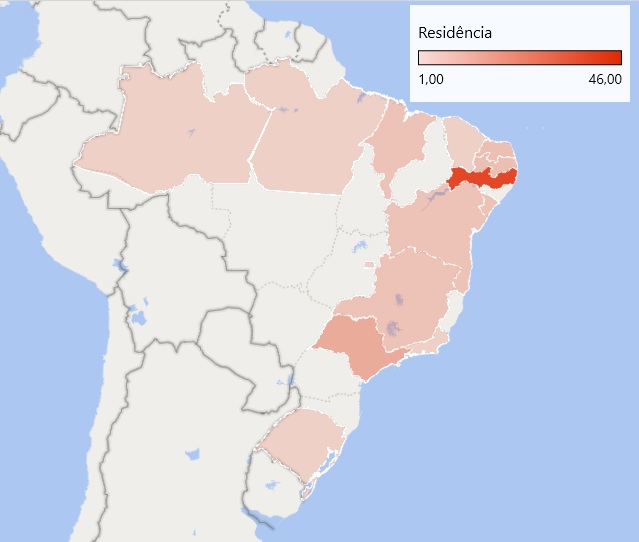
\includegraphics[width=12cm]{images/residencia.jpg}
    \caption{Mapa de densidade demográfica dos participantes}
    \label{fig:residencia}
\end{figure}


\begin{table}[H]
\centering
\caption{Local onde residem os participantes}
\label{tab:residencias}
\begin{tabular}{|c|c|}
\hline
UF            & QUANTIDADE \\ \hline
\rowcolor[HTML]{FFCCC9} 
AM            & 1             \\ \hline
\rowcolor[HTML]{FFCCC9} 
PA            & 1             \\ \hline
\rowcolor[HTML]{FFFC9E} 
BA            & 2             \\ \hline
\rowcolor[HTML]{FFFC9E} 
CE            & 1             \\ \hline
\rowcolor[HTML]{FFFC9E} 
MA            & 2             \\ \hline
\rowcolor[HTML]{FFFC9E} 
PB            & 3             \\ \hline
\rowcolor[HTML]{FFFC9E} 
PE            & 45            \\ \hline
\rowcolor[HTML]{FFFC9E} 
RN            & 3             \\ \hline
\rowcolor[HTML]{FFFC9E} 
SE            & 2             \\ \hline
\rowcolor[HTML]{9AFF99} 
DF            & 1             \\ \hline
\rowcolor[HTML]{CBCEFB} 
MG            & 1             \\ \hline
\rowcolor[HTML]{CBCEFB} 
RJ            & 1             \\ \hline
\rowcolor[HTML]{CBCEFB} 
SP            & 11            \\ \hline
\rowcolor[HTML]{34CDF9} 
RS            & 1             \\ \hline
\rowcolor[HTML]{C0C0C0} 
Estrangeiro   & 2             \\ \hline
Não Declarado & 1             \\ \hline
TOTAL         & 78            \\ \hline
\end{tabular}
\end{table}
